\documentclass[12pt]{scrartcl}

\usepackage[utf8]{inputenc}
\usepackage[T1]{fontenc}
\usepackage{lmodern}
\usepackage{graphicx}
\usepackage[pdftex,hyperref,dvipsnames]{xcolor}
\usepackage{listings}
\usepackage[a4paper,lmargin={2cm},rmargin={2cm},tmargin={3.5cm},bmargin = {2.5cm},headheight = {4cm}]{geometry}
\usepackage{amsmath,amssymb,amstext,amsthm}
% \usepackage[lined,algonl,boxed]{algorithm2e} 
\usepackage{algpseudocode}
\usepackage{tikz}
\usepackage{pgfplots}
\usepackage{hyperref}
\usepackage{url}
\usepackage{tcolorbox}
\usepackage{float}
\usepackage[inline]{enumitem}
\usepackage[headsepline]{scrlayer-scrpage} 

\usetikzlibrary{automata,positioning}

\usepgfplotslibrary{external}
%\tikzexternalize
\pgfplotsset{width=10cm,compat=1.9}
\pgfplotsset{every axis/.style={
    axis line style = thick,
    grid = both,
    tick pos = left,
    tick align = outside,
    tick style = {thick,black},
    fill = blue,
	line width = 2pt,
}}

\lstset{
  basicstyle=\ttfamily\small,
  numbers=left,
  numberstyle=\tiny,
  stepnumber=1,
  numbersep=8pt,
  frame=single,
  breaklines=true,
  columns=fullflexible
}

\lstset{
  language=C,
  basicstyle=\ttfamily\small,
  keywordstyle=\color{blue},
  commentstyle=\color{gray},
  stringstyle=\color{green!60!black},
  numbers=left,
  numberstyle=\tiny,
  stepnumber=1,
  numbersep=8pt,
  frame=single,
  breaklines=true,
  columns=fullflexible
}

\renewcommand{\theenumi}{(\alph{enumi})}
\renewcommand{\labelenumi}{\text{\theenumi}}
\renewcommand{\labelenumii}{(\roman{enumii})} 

\ohead{Weiting Wang (3855168)\\
       Nico Strohbach (3546914)\\
       Jan Theil (3794698)}

\ihead{Reinforcement Learning}

\newcounter{exnum}
\newcommand{\exercise}[1]{\section*{Problem \theexnum\stepcounter{exnum}: #1}}

\begin{document}

\setcounter{exnum}{1}
\exercise{Monte Carlo Methods vs Dynamic Programming}

\begin{enumerate}
  \item \begin{itemize}
          \item The agent can learn directly from experience. Hence, they can learn in real time interacting with the environment.
          \item No need to model the whole environment ($p(\cdot)$).
        \end{itemize}
  \item One example would be the humanoid house chore roboter. The environment (action-state set) is way too big to run dynamic programming on. The environment changes, too, which could be handled on-the-fly using MC methods.
\end{enumerate}

\exercise{Monte Carlo ES for blackjack}

\begin{enumerate}
  \item For the code, please check \textit{ex04-mc.py}.
        \begin{figure}[H]
          \centering
          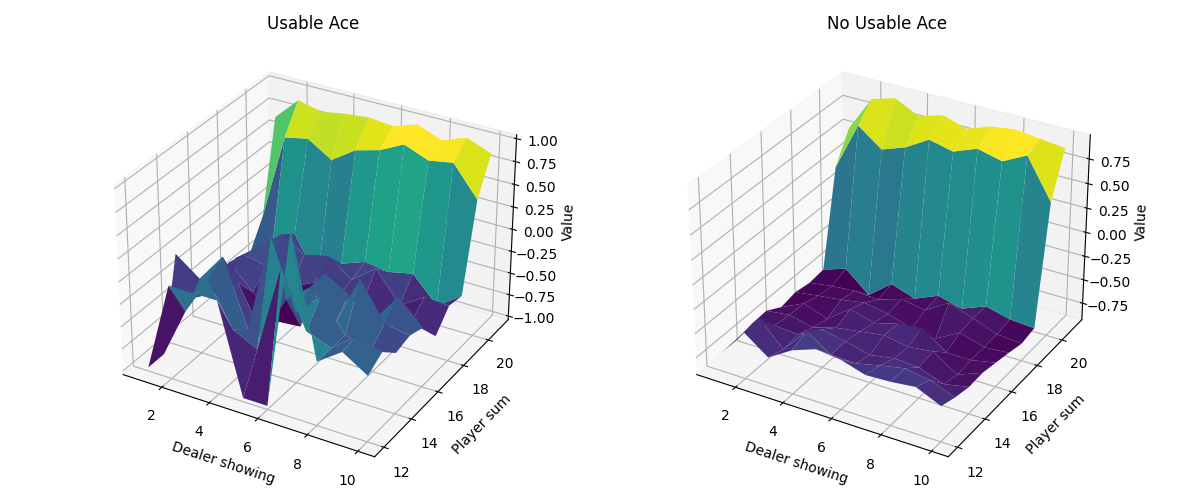
\includegraphics[width=\textwidth]{MC10000.png}
          \caption{After 10,000 episodes}
          \label{fig:MC10000}
        \end{figure}

        \begin{figure}[H]
          \centering
          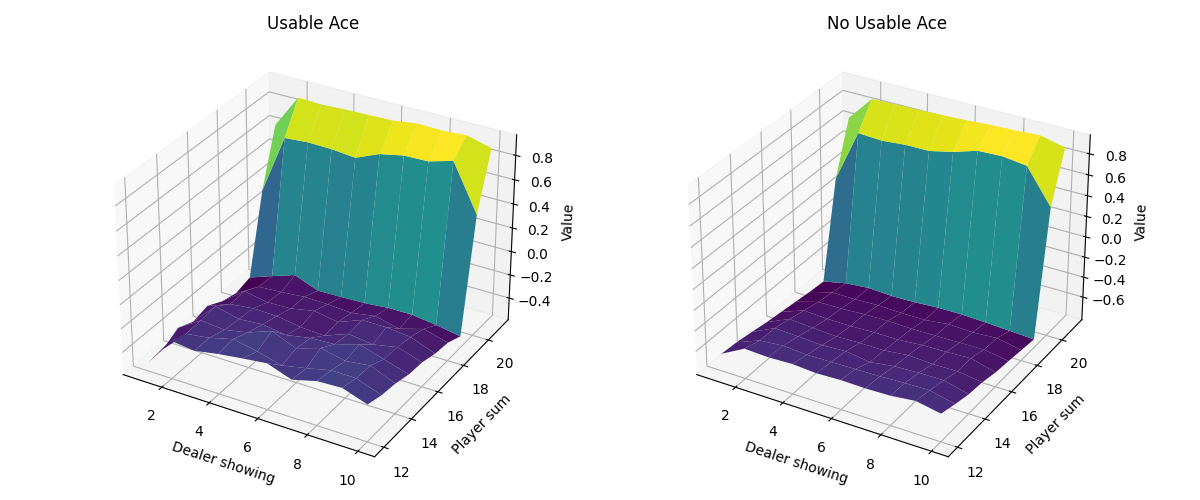
\includegraphics[width=\textwidth]{MC500000.png}
          \caption{After 500,000 episodes}
          \label{fig:MC500000}
        \end{figure}
  \item The plots show the learned state-value function for Blackjack using Monte Carlo Exploring Starts.
  Higher values correspond to states with a higher expected reward.
  States with high player sums (20–21) generally have positive values, especially when the dealer shows a low card.
  States with low player sums or strong dealer cards have lower values.
  The value function with a usable ace is generally higher because the ace provides more flexibility and reduces the probability of busting.
        \begin{figure}[H]
          \centering
          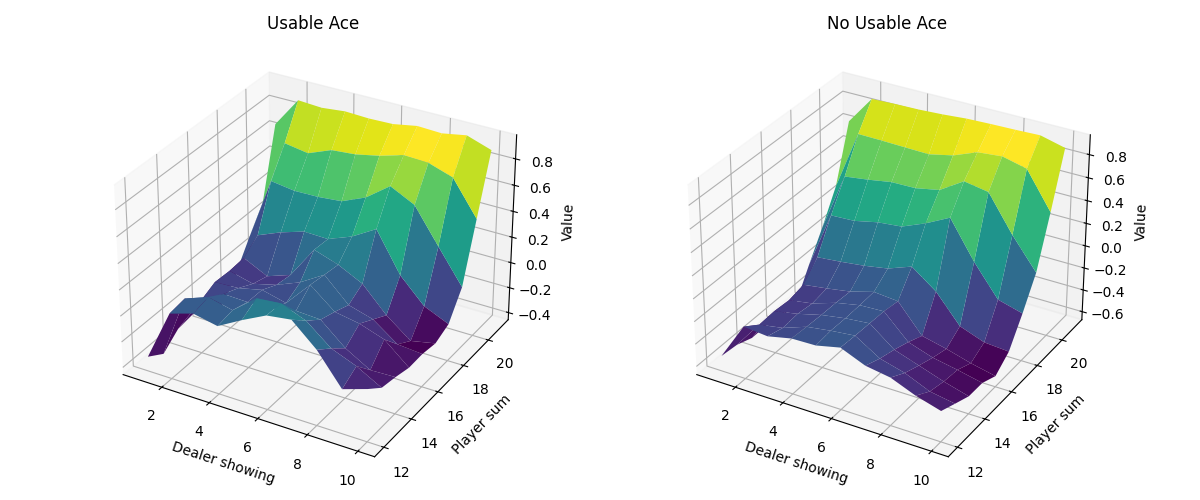
\includegraphics[width=\textwidth]{MonteCarlo_2b.png}
          \caption{After 500,000 iterations}
          \label{fig:MonteCarlo_2b}
        \end{figure}
  The following tables show the final policy $\pi(s)$ learned using Monte Carlo Exploring Starts.  
  Action encoding: 0 = stick, 1 = hit. X-Axis: dealer's showing card (1-10), Y-Axis: player's current sum (12-21).

  \subsubsection*{Usable Ace}

  \begin{table}[h]
  \centering
  \scriptsize
  \texttt{
    \begin{tabular}{c|cccccccccc}
        & 1 & 2 & 3 & 4 & 5 & 6 & 7 & 8 & 9 & 10 \\
    \hline
    12 & 1 & 1 & 1 & 1 & 1 & 1 & 1 & 1 & 1 & 1 \\
    13 & 1 & 1 & 1 & 1 & 1 & 1 & 1 & 1 & 1 & 1 \\
    14 & 1 & 1 & 1 & 1 & 1 & 1 & 1 & 1 & 1 & 1 \\
    15 & 1 & 1 & 1 & 1 & 1 & 1 & 1 & 1 & 1 & 1 \\
    16 & 1 & 1 & 1 & 1 & 1 & 1 & 1 & 1 & 1 & 1 \\
    17 & 1 & 1 & 1 & 1 & 1 & 1 & 1 & 1 & 1 & 1 \\
    18 & 1 & 0 & 0 & 0 & 1 & 0 & 0 & 0 & 1 & 1 \\
    19 & 0 & 0 & 0 & 0 & 0 & 0 & 0 & 0 & 0 & 0 \\
    20 & 0 & 0 & 0 & 0 & 0 & 0 & 0 & 0 & 0 & 0 \\
    21 & 0 & 0 & 0 & 0 & 0 & 0 & 0 & 0 & 0 & 0 \\
    \end{tabular}
    }
  \caption{Policy with usable ace}
  \end{table}

  \subsubsection*{No Usable Ace}

  \begin{table}[h]
  \centering
  \scriptsize
  \texttt{
    \begin{tabular}{c|cccccccccc}
        & 1 & 2 & 3 & 4 & 5 & 6 & 7 & 8 & 9 & 10 \\
    \hline
    12 & 1 & 1 & 1 & 0 & 0 & 0 & 1 & 1 & 1 & 1 \\
    13 & 1 & 1 & 0 & 0 & 0 & 0 & 1 & 1 & 1 & 1 \\
    14 & 1 & 0 & 0 & 0 & 0 & 0 & 1 & 1 & 1 & 1 \\
    15 & 1 & 0 & 0 & 0 & 0 & 0 & 1 & 1 & 1 & 1 \\
    16 & 1 & 0 & 0 & 0 & 0 & 0 & 1 & 1 & 0 & 1 \\
    17 & 0 & 0 & 0 & 0 & 0 & 0 & 0 & 0 & 0 & 0 \\
    18 & 0 & 0 & 0 & 0 & 0 & 0 & 0 & 0 & 0 & 0 \\
    19 & 0 & 0 & 0 & 0 & 0 & 0 & 0 & 0 & 0 & 0 \\
    20 & 0 & 0 & 0 & 0 & 0 & 0 & 0 & 0 & 0 & 0 \\
    21 & 0 & 0 & 0 & 0 & 0 & 0 & 0 & 0 & 0 & 0 \\
    \end{tabular}
    }
  \caption{Policy without usable ace}
  \end{table}


\end{enumerate}

\end{document}